\documentclass[tikz,border=8pt]{standalone}
\usetikzlibrary{arrows.meta,fit,backgrounds,positioning,calc}
\begin{document}
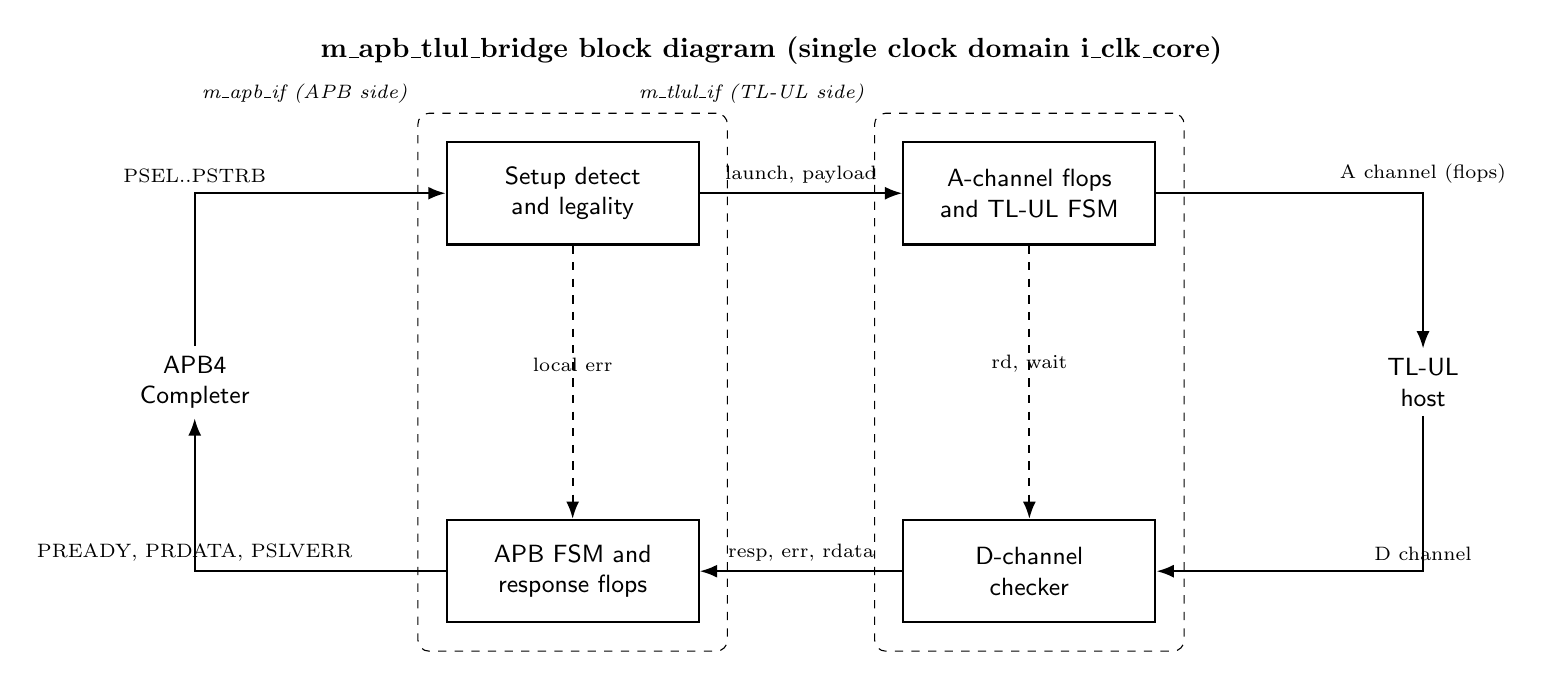
\begin{tikzpicture}[font=\sffamily\small,
  blk/.style={draw,thick,minimum width=3.2cm,minimum height=1.3cm,align=center,fill=white},
  mem/.style={blk,double,double distance=1.5pt},
  clk/.style={blk,rounded corners=6pt},
  io/.style={align=center,minimum width=1.6cm,minimum height=0.8cm},
  data/.style={-{Latex[length=2.2mm]},thick},
  ctrl/.style={-{Latex[length=2.2mm]},thick,dashed},
  clock/.style={-{Latex[length=2.2mm]},thick,dotted}]
\node[io] (io_apb) at (0.00,-2.40) {APB4\\ Completer};
\node[blk] (dec) at (4.80,0.00) {Setup detect\\ and legality};
\node[blk] (arsp) at (4.80,-4.80) {APB FSM and\\ response flops};
\node[blk] (tla) at (10.60,0.00) {A-channel flops\\ and TL-UL FSM};
\node[blk] (tld) at (10.60,-4.80) {D-channel\\ checker};
\node[io] (io_tl) at (15.60,-2.40) {TL-UL\\ host};
\draw[data] (io_apb.north) |- node[midway,above,font=\scriptsize,align=center]{PSEL..PSTRB} (dec.west);
\draw[data] (dec.east) -| ($(dec.east)!.5!(tla.west)$) |- node[midway,above,font=\scriptsize,align=center]{launch, payload} (tla.west);
\draw[data] (tla.east) -| node[midway,above,font=\scriptsize,align=center]{A channel (flops)} (io_tl.north);
\draw[data] (io_tl.south) |- node[midway,above,font=\scriptsize,align=center]{D channel} (tld.east);
\draw[data] (tld.west) -| ($(tld.west)!.5!(arsp.east)$) |- node[midway,above,font=\scriptsize,align=center]{resp, err, rdata} (arsp.east);
\draw[data] (arsp.west) -| node[midway,above,font=\scriptsize,align=center]{PREADY, PRDATA, PSLVERR} (io_apb.south);
\draw[ctrl] (dec.south) |- ($(dec.south)!.5!(arsp.north)$) -| node[midway,above,font=\scriptsize,align=center]{local err} (arsp.north);
\draw[ctrl] (tla.south) |- ($(tla.south)!.5!(tld.north)$) -| node[midway,above,font=\scriptsize,align=center]{rd, wait} (tld.north);
\begin{scope}[on background layer]
\node[draw,dashed,rounded corners=4pt,inner sep=10pt,fit=(dec)(arsp),label={[font=\scriptsize\itshape]north west:m\_apb\_if (APB side)}] (g0) {};
\node[draw,dashed,rounded corners=4pt,inner sep=10pt,fit=(tla)(tld),label={[font=\scriptsize\itshape]north west:m\_tlul\_if (TL-UL side)}] (g1) {};
\end{scope}
\node[font=\bfseries,anchor=south] at (current bounding box.north) {m\_apb\_tlul\_bridge block diagram (single clock domain i\_clk\_core)};
\end{tikzpicture}
\end{document}
